%{\setbeamercolor{background canvas}{bg=felix_bg}
\begin{frame}[t]
	\frametitle{Complexity}
		Can we determine if a problem with $n$ items is poly-time solvable?
		\vspace{1.0cm}
		\begin{itemize}
			\item An $n^{O(1)}$ algorithm: Problem is solved!
			\vspace{1.0cm}
			\item NP-Hard: Not poly-time solvable assuming $P \neq NP$.
		\end{itemize}
\end{frame}

\begin{frame}[t]
	\frametitle{Parameterized Complexity}
	What if our problem has an additional parameter $k$ s.t. $n >> k$?
	\vspace{1.0cm}
	\begin{itemize}
		\item FPT: There exists an algorithm that runs in $O(f(k)n^{O(1)})$ time.
		\vspace{1.0cm}
		\item W[1]-Hard: No FPT algorithm exists assuming $FPT \neq XP$.
		\vspace{1.0cm}
		\item XP: There exists an algorithm that runs in $O(n^{f(k)})$ time.
	\end{itemize}
\end{frame}

\begin{frame}[t]
	\frametitle{Gerrymandering in Practice}
	% Note: some image here going from a few states in the US to an actual graph.
	Gerrymandering is the process of manipulating districts in an election in order for a desired candidate to win.
	\vspace{0.5em}

			\begin{figure}
				\begin{center}
					\includegraphics[scale=0.275]{figures/ut_gm.pdf}
				\end{center}
			\end{figure}
			{\let\thefootnote\relax\footnote{{Source: redistricting.lls.edu}}}
\end{frame}

\begin{frame}[t]
	\frametitle{Defining Gerrymandering}
	\small
	\problembox{Gerrymandering}
	{A graph $G = (V,E)$, a set of candidates $C$, a candidate function $\chi: V \rightarrow C$, a weight function $w: V \rightarrow \mathbb{N}$, a preferred candidate $p \in C$, and an integer $k \in \mathbb{N}$.}
	{Is there a district-partition of $V$ into $k$ districts such that $p$ wins more districts than any other candidate?}

	\onslide<2> {
			\begin{figure}
				\begin{center}
					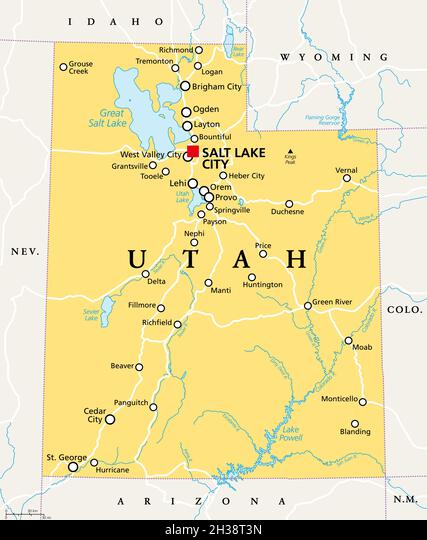
\includegraphics[scale=0.15]{figures/ut.jpg}
					\begin{tikzpicture}
    \tikzstyle{node} = [circle, draw, thick, minimum size=0.7cm]
	\tikzstyle{edge} = [thick]

    \node (u00) [node] {};
    \node (u01) [node, right=0.2cm of u00] {};
    \node (u1) [node, below=0.2cm of u00] {};
    \node (u2) [node, right=0.2cm of u1] {};
    \node (u3) [node, right=0.2cm of u2] {};
    \node (u4) [node, right=0.2cm of u3] {};
    \node (u5) [node, below=0.2cm of u1] {};
    \node (u6) [node, right=0.2cm of u5] {};
    \node (u7) [node, right=0.2cm of u6] {};
    \node (u8) [node, right=0.2cm of u7] {};
    \node (u9) [node, below=0.2cm of u5] {};
    \node (u10) [node, right=0.2cm of u9] {};
    \node (u11) [node, right=0.2cm of u10] {};
    \node (u12) [node, right=0.2cm of u11] {};

    \node (p1) [above left = 0.1cm and 0.3cm of u5] {};
    \node (p2) [left = 1.0cm of p1] {};
    \draw[->, ultra thick, color=black] ($(p2) + (0.0, 0.0)$) -> ($(p1) + (0.0, 0.0)$);

    \draw (u00) edge [edge] (u01);
    \draw (u1) edge [edge] (u2);
    \draw (u2) edge [edge] (u3);
    \draw (u3) edge [edge] (u4);
    \draw (u5) edge [edge] (u6);
    \draw (u6) edge [edge] (u7);
    \draw (u7) edge [edge] (u8);
    \draw (u9) edge [edge] (u10);
    \draw (u10) edge [edge] (u11);
    \draw (u11) edge [edge] (u12);
    \draw (u00) edge [edge] (u1);
    \draw (u01) edge [edge] (u2);
    \draw (u1) edge [edge] (u5);
    \draw (u2) edge [edge] (u6);
    \draw (u3) edge [edge] (u7);
    \draw (u4) edge [edge] (u8);
    \draw (u5) edge [edge] (u9);
    \draw (u6) edge [edge] (u10);
    \draw (u7) edge [edge] (u11);
    \draw (u8) edge [edge] (u12);

\end{tikzpicture}
				\end{center}
			\end{figure}
	}
\end{frame}

\begin{frame}[t]
	\frametitle{Gerrymandering Example}
	\begin{figure}
		\begin{center}
			
\begin{tikzpicture}
	\tikzstyle{node} = [circle, draw, thick]
	\tikzstyle{edge} = [thick]

	\node (1) [node, fill=orange] {4};
	\node (2) [node, fill=orange, right=0.6cm of 1] {2};
	\node (3) [node, fill=skyblue, right=0.6cm of 2] {5};
	\node (4) [node, fill=orange, above=0.5cm of 2] {2};

	\node (5) [node, fill=bluegreen, below right=0.45cm and 0.3cm of 3] {3};
	\node (6) [node, fill=bluegreen, below right=0.5cm and 0.2cm of 1] {1};
	\node (12) [node, fill=bluegreen, below right=0.5cm and 0.2cm of 5] {7};

	\node (9) [node, fill=skyblue, below left=0.5cm and 0.2cm of 1] {4};
	\node (10) [node, fill=skyblue, below left=0.5cm and 0.1cm of 9] {2};
	\node (11) [node, fill=orange, below right=0.5cm and 0.1cm of 9] {5};

	\draw (1) edge [edge] (4);
	\draw (1) edge [edge] (6);
	\draw (1) edge [edge] (9);
	\draw (2) edge [edge] (4);
	\draw (3) edge [edge] (5);
	\draw (3) edge [edge] (4);

	\draw (9) edge [edge] (10);
	\draw (11) edge [edge] (9);
	\draw (12) edge [edge] (5);

	\tikzstyle{node} = []

	\onslide<2-3> {
		\node (phint) [node, text=skyblue, above left=0.8cm and 0.3cm of 10] {$p$: 6 votes};
		\node (ohint) [node, text=orange, above left=0.4cm and 0.3cm of 10] {orange: 5 votes};
		\node (distresult) [node, above left=0cm and 0.3cm of 10] {$p$ wins!};
		\draw[ultra thick, rounded corners=6mm, color=skyblue] ($(9.north)+(0,0.5)$) -- ($(10.south west)+(-0.5,-0.2)$) -- ($(11.south east)+(0.5,-0.2)$) -- cycle;
	}

	\onslide<3> {
		\draw[ultra thick, rotate=-55, rounded corners, color=orange] ($(1.north west)+(-0.1,0.45)$) rectangle ($(6.south east)+(0.1, -0.45)$);

		\draw[ultra thick, rounded corners=10mm, color=skyblue] ($(4.north west)+(-0.1,0.7)$) -- ($(2.south west)+(-0.4,-0.4)$) -- ($(3.south east)+(0.7,-0.1)$) -- cycle;

		\draw[ultra thick, rotate=-55, rounded corners, color=bluegreen] ($(5.north west)+(-0.1, 0.45)$) rectangle ($(12.south east)+(0.1, -0.45)$);
	}
	
	

\end{tikzpicture}

		\end{center}
	\end{figure}

	\begin{itemize}
		\item Candidates $\rightarrow$ color. Our preferred candidate $p$ is blue.
		\item Weights $\rightarrow$ votes.
		\onslide<3> {
			\item Our candidate $p$ wins twice, others win once. Therefore, this is a YES-instance.
			\item This instance has $k=4$ districts.
		}
	\end{itemize}
\end{frame}